\chapter{Overview of Publications}
\label{ch:overview_of_publications}

This chapter provides an introduction and overview to the five publications included in this compendium thesis. As mentioned above, two of the publications, [P1] and [P2], are excerpted from the book \emph{Geospatial Computing in Mobile Devices}, published by Artech House in 2014. Two others, [P3] and [P4], were published in the peer-reviewed open access journal \emph{Sensors}. The final publication [P5] was published in the Proceedings of the \gls{plans}, jointly organized by the \gls{aess} and the \gls{ion}. AESS is an affiliate society of the \gls{ieee}.

The remainder of this chapter is organized as follows: Section~\ref{sec:overall_research} describes the overall research goals and research setting under which the publications were prepared. Section~\ref{sec:relating_to_research} maps the included publications to the overall research goals presented in this thesis. Section~\ref{sec:author_contributions} describes the author's contributions to each publication. Finally, Section~\ref{sec:impact} outlines the scientific impact of the included publications.

\section{Research Context for Publications}
\label{sec:overall_research}

The overall research goal of this thesis was stated in Chapter~\ref{ch:intro}: to improve our understanding of how computing devices can better understand us and our needs. Also, the detailed research objectives were summarized in Section~\ref{sec:objectives} in terms of three specific tasks. Nonetheless, in this section, we aim to describe the broader research context (no pun intended) in which the five included publications were prepared and written, in order to better frame the publications and understand their interrelationships.

Firstly, a significant focus of our overall research portfolio during the years 2011--2013 was making the transition from growing ubiquitous positioning capabilities in mobile devices to emerging context awareness capabilities. This research focus was especially evident in the project ``\acrlong{inosense}'' (\acrshort{inosense}), funded by the Academy of Finland. The goal of this project was ``to carry out research on sensing social context, modeling human behavior and developing a new mobile architecture for social applications'' \cite{inosense2015}. It is primarily within this project that the research described in publications [P3] and [P4] was prepared.

During the INOSENSE project, we decided to initiate an ambitious book project. The book, \emph{Geospatial Computing in Mobile Devices}, written jointly by Prof. Ruizhi Chen and the author of this thesis, was prepared to present our ongoing research work and other efforts in the field of mobile geospatial computing. The intended audience was not only the scientific community but also potential engineers and developers who may be interested in putting the research results into practice. In particular, the two chapters included in this thesis cover the topic of context awareness, a key topic in this thesis. Preparing these book chapters also provided an excellent opportunity to carry out a detailed literature review on the topic of context awareness. Overall, the book was prepared between May 2012 and March 2014 during the author's spare time, alongside INOSENSE and other project responsibilities. 

One of overall goals of covering context awareness in ``textbook format'' was to help raise the profile of context awareness within the mobile computing and geospatial sciences communities. We are aware of no other book in the field of mobile geospatial computing that covers also context awareness, and there are very few books overall that cover context awareness to any significant depth.  We believe that the growing capabilities of smart mobile devices, such as the smartphone, present a potentially breakthrough opportunity for context awareness to become an important topic in these research communities.

In August 2013, the author transitioned to a new project with rather different research goals. The name of the project was ``\acrlong{arcsat}'' or acrshort{arcsat} for short. Although the project included many different research topics, our research goal in the project was to carry out a feasibility study on the development of an ``ice-aware'' navigation solution for Arctic seas. It was stated in the project plan that ``...awareness of the sea ice and sea weather information will improve the safety of the navigation solution especially in Arctic areas.'' Although the application area is clearly very different from that of the INOSENSE project, the concept of context awareness was evidently relevant. One other difference between the two projects is that in INOSENSE, the main focus was on \emph{generating} context awareness, whereas applications of context awareness were largely out of scope. By contrast, in ARCSAT the focus was more on utilizing context awareness---in particular ice awareness---for navigation purposes. The main output of the project was publication [P5]. In addition, this project bore fruit in terms of two related research projects which were initiated in 2015.

In about March 2014, the author again transitioned to a new project, called \acrshort{esabalt}, which continued our line of research related to maritime navigation. The research results of this project, however, are outside the scope of this thesis and will not be discussed further. These project transitions are the main reason for the gap of more than two years between publications [P3] and [P4], despite the fact that they cover related topics.

\section{Mapping of Publications to Research Areas}
\label{sec:relating_to_research}

Figure~\ref{fig:publication-chart} presents a mapping between the included publications [P1]-[P5] and different areas of research within the topic of context awareness. These areas can be divided into three broad areas: (1) background and literature review, (2) concepts and theory, and (3) different use case scenarios. Publications [P1] and [P2] fall primarily within the first and second areas, respectively. Publications [P3]-[P5], although containing some elements from the first two areas, mainly deal with different use case scenarios where context awareness can be applied.

\begin{figure}
  \begin{center}
    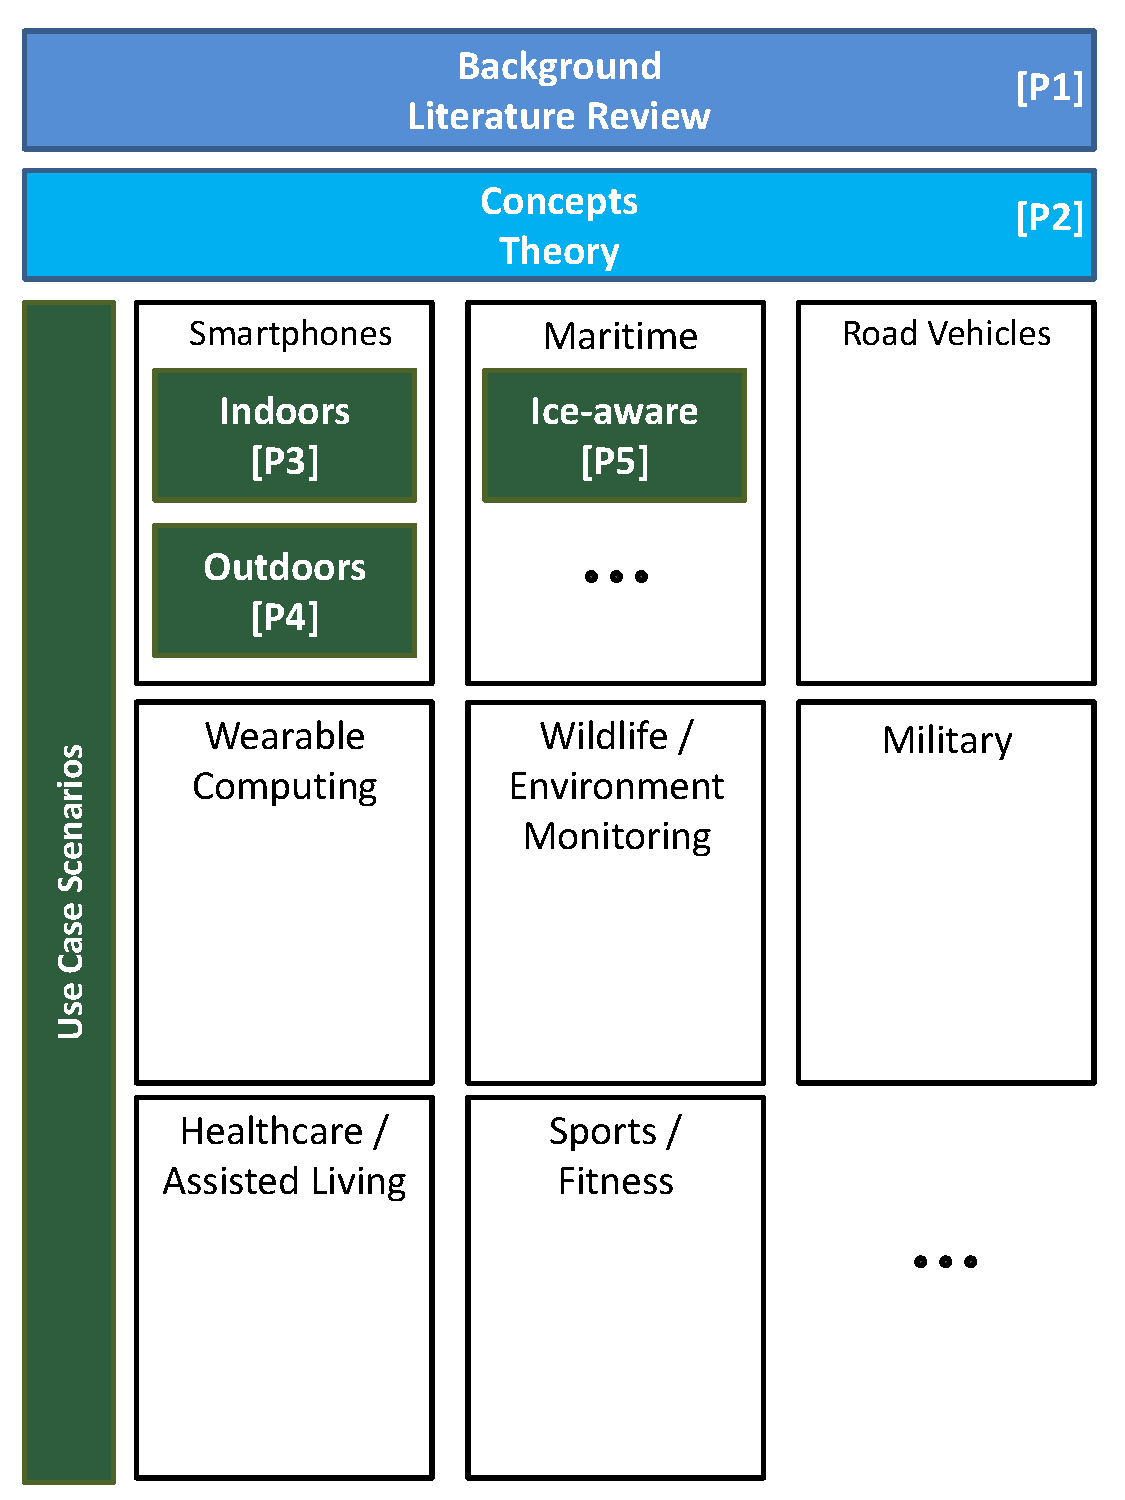
\includegraphics[width=1.0\textwidth]{Images/figChapter4}
  \end{center}
  \caption[Mapping of included publications to research areas]{Mapping of included publications to research areas. The additional empty boxes are indtended to emphasize that many use case scenarios have yet to be explored. Further discussion on future use case scenarios can be found in Section~\ref{sec:future_applications}.}
  \label{fig:publication-chart}
\end{figure}

As the Figure~\ref{fig:publication-chart} indicates, there are many potential use case scenarios that are not addressed in this thesis. There are, of course, many possible ways to categorize and sub-categorize the use cases, and this chart is not intended to be authoritative in this matter. The list is also not exhaustive. Our original research plan was to cover as many different use case scenarios as possible, but due to time constraints and project limitations, only two separate use case scenarios could be investigated (or three, if you consider [P3] and [P4] to cover separate use case scenarios). Our plans to cover additional use case scenarios will be discussed briefly in Chapter~\ref{ch:conclusions}.


\section{Author's Contributions to the Publications}
\label{sec:author_contributions}

This section outlines the main contributions of the author of this thesis to the included publications.

\textbf{[P1]:} The thesis author was the main author of this chapter, whereas the book co-author provided only editorial comments to a near-final draft. The thesis author conducted all the necessary background literature review and independently decided on the detailed contents of the chapter. The author also came up with the idea to use Hermagoras's ``seven elements of circumstance'' to organize and describe the different elements of context. The author also independently identified and collated the various Android Application Programming Interfaces (APIs) relevant to context awareness.

\textbf{[P2]:} The thesis author was the main author of this chapter, whereas the book co-author provided only editorial comments to a near-final draft. Similar to [P1] thesis author conducted all the necessary background literature review and independently decided on the detailed contents of the chapter. The author created all of the figures in the chapter and originated the concept of the ``context pyramid''. Finally, one of the main contributions of this chapter is the formulation and description (including figures) of rather somewhat complex mathematical concepts (e.g. \acrlong{svm}) in such a way that they are understandable to anyone with basic knowledge in algebra and probability.

\textbf{[P3]:} The thesis author was the second author of this publication, but the first author has affirmed in writing that the thesis author's contribution was roughly equal to that of the thesis author. The thesis author contributed equally to the design and implementation of the experiments, including implementation of the data collection application on a smartphone. He assisted in the analysis of the test results. Also, he was the originator of the idea used for indoor-outdoor detection based on GPS signal-to-noise ratio and WiFi signal strength and implemented this method in a smartphone. The thesis author contributed to the development of the WiFi fingerprinting indoor positioning system and prepared the test environment by measuring and marking reference points and setting up additional WiFi access points. As stated earlier, he was the originator of the ``context pyramid'' concept, which is also described and employed in this paper. He was also the originator of the idea of using a graph-based grouping of the reference points. Lastly, he contributed to the preparation of the manuscript, including writing some sections and editing it in its entirety.

\textbf{[P4]:} The thesis author was the sole author of this publication and received assistance only in the data collection part, as well as general guidance form his supervisors. He also implemented all the necessary software used in the experiments, apart from the Weka software platform used in the data analysis. Some extensions to Weka, in terms of automating analysis and integrating Weka with Matlab, were also implemented by the author.

\textbf{[P5]:} The thesis author was the first author of this publication and was the originator of the idea of using a graph-based approach and the A* algorithm for ice-aware route optimization. He implemented the optimization algorithm in Matlab, basing the implementation only roughly on an open source implementation. He also designed the graph structure, in terms of optimizing the discretization of the ship's motion model. The only parts of the implementation that were not done by the thesis author were the implementation of the resistive ship speed model, representation of the ice data, and provision of the historical ship data, all of which were provided by co-authors. Finally, the thesis author led the manuscript preparation, writing most sections, preparing all figures, and editing the manuscript in its entirety.

\section{Scientific Impact of the Publications}
\label{sec:impact}

Perhaps the most straightforward approach to measuring the scientific impact of publications is via citations in other scientific works. All of the included publications have received multiple citations, and Table~\ref{table:citations} shows these statistics. Data is provided mostly by the Google Scholar service and has been supplemented with a few missing citations that were known to the author. All citations have been manually checked for accuracy. In the case of [P4], this statistic includes, in fact, citations from two related publications. [P4] was first published in shorter form in 2013 as a conference paper \cite{Guinness2013}, and it was only recently (April, 2015) published as a journal article. Thus, it seems fitting that citations from \cite{Guinness2013} are included as well. We note also that \cite{Guinness2013} received the Student Paper Award of the conference where it was presented.
%
\begin{table}
\centering
\begin{tabular}{ccc}
\hline\noalign{\smallskip}
\textbf{Publication} & \textbf{Year} & \textbf{\# of Citations}\\
\hline\noalign{\smallskip}
P1 & 2014 & 4\\
P2 & 2014 & 4\\
P3 & 2013 & 20\\
P4 & 2015 & 5\\
P5 & 2014 & 2\\
\hline\noalign{\smallskip}
\end{tabular}
\caption[Citation statistics for included publications]{Statistics on the number of citations for each of the included publications. Data come mostly from Google Scholar and the author's own records.}\label{table:citations}
\end{table}
%
In addition to citations, the published work has had the result that the author has been invited to participate in the peer review process for several scientific articles on related topics. He has also been invited to serve on a scientific panel at the 2015 ION GNSS+ conference.

Several of the included publications appear in scientific forums that have been rated by the Finnish Publication Forum (in Finnish: Julkaisufoorumi, abbreviated \acrshort{jufo}) \cite{jufo}. At the time of their publication, these forums had the following ratings:

\begin{itemize}
  \setlength\itemsep{0em}
  \item[] [P1]: JuFo Level 1
  \item[] {[P2]}: JuFo Level 1
  \item[] {[P3]}: JuFo Level 1
  \item[] {[P4]}: JuFo Level 1
  \item[] {[P5]}: Not rated by JuFo
\end{itemize}


Lastly, [P5] was nominated by a peer reviewer for the Walter R. Fried Memorial Award for best paper of the conference.



